\section{ParSplice Keyspace Analysis}
%IT HAS 8K keys!  How did we take these measurements

We instrumented ParSplice with performance counters and keyspace counters.  The
performance counters track ParSplice activities while keyspace counters track
which keys were being accessed by the ranks. Because the keyspace counters have
high overhead we only turn them on for the keyspace analysis.

The cache hierarchy was unmodified but for the backend persistent database, we
replaced BerkeleyDB on NFS with LevelDB on Lustre. Original ParSplice
experiments showed that BerkeleyDB's syncs caused reads/writes to pile up on
the persistent database node. We also use Riak's customized
LevelDB\footnote{https://github.com/basho/leveldb} version, which comes
instrumented with its own set of performance counters.

\subsection*{Testbed: Cray XC40}

All experiments were run on Trinitite, a Cray XC40 with 100 nodes each with 32
Intel Haswell 2.3GHz cores.  Each node has 128GB of RAM and our goal is to
limit the size of the database to 3\% of RAM. Note that this is an addition to
the 30GB that ParSplice uses to manage other ranks on the same node. 

Inititial runs on commodity hardware, 10 CloudLab nodes and 10 nodes in our
private cluster, show poor performance compared to the Cray. A single Cray node
produces trajectories that are \(45\times)\) longer than our CloudLab clusters
and \(24\times\) longer than our own cluster. As a result, it reaches different
job phases faster and gives us a more comprehensive view of the workload. The
performance gains compared to the commodity clusters has more to do with
memory/PCI bandwidth than network.

\subsection*{Results}
We examine the keyspace size and access patterns using
Figures~\ref{fig:futurework-regimes} and~\ref{fig:methodology-keyspace}.

\subsubsection*{An active but small keyspace} The black text annotations in
Figure~\ref{fig:methodology-keyspace} show that the keyspace size ranges from
about 10K keys for 32 workers to 100K keys for 1048 workers.  The bars show
\(50-100\times\) as many reads (\texttt{get()}) as writes (\texttt{put()}).
Workers read the same key for extended periods because the trajectory segment
is stuck in a superbasin composed of local minima, so many coordinates are
needed before the trajectory moves on. Writes only occur for the final state of
segments generated by workers; their magnitude is smaller than reads because
the caches ignore redundant put requests. The number of read and write requests
are highest at the beginning of the run when workers generate segements for the
same state, which is cheap. This type of keyspace encourages replication across
a cluster.  

\subsubsection*{Entropy increases over time} The reads per second in
Figure~\ref{fig:futurework-regimes} show that the number of requests decreases
and the number of active keys increases over time. The resulting imbalance for
the two growth rates in Figure~\ref{fig:futurework-regimes} are shown in
Figure~\ref{fig:methodology-keys}, where reads are plotted for each unique
state (\(x\) axis). Keys are more popular than others (up to \(5\times\))
because workers start generating states with different coordinates later in the
run.

\subsubsection*{Entropy growth is structured} The access patterns reflect the
locality of computation: workers stuck in state basins generate segments with
similar coordinates. The growth rate, temperature, and number of workers
changes that locality, which has an effect on the structure of the keyspace.
Figure~\ref{fig:methodology-keys} shows that the number of reads changes with
different growth rates, but that spatial locality is similiar ({\it e.g.}, some
keys are stil \(5\times\) more popular than others).
Figure~\ref{fig:futurework-regimes} shows how entropy for different growth
rates has temporal locality, as the reads per second for 1M looks like the
reads per second for 100K stretched out along the time axis.  Trends also exist
for temperature and number of workers but are ommitted here for space. This
structure means that we can learn the regimes and adapt the storage system to
it. 

\begin{figure}[tbh]
  \noindent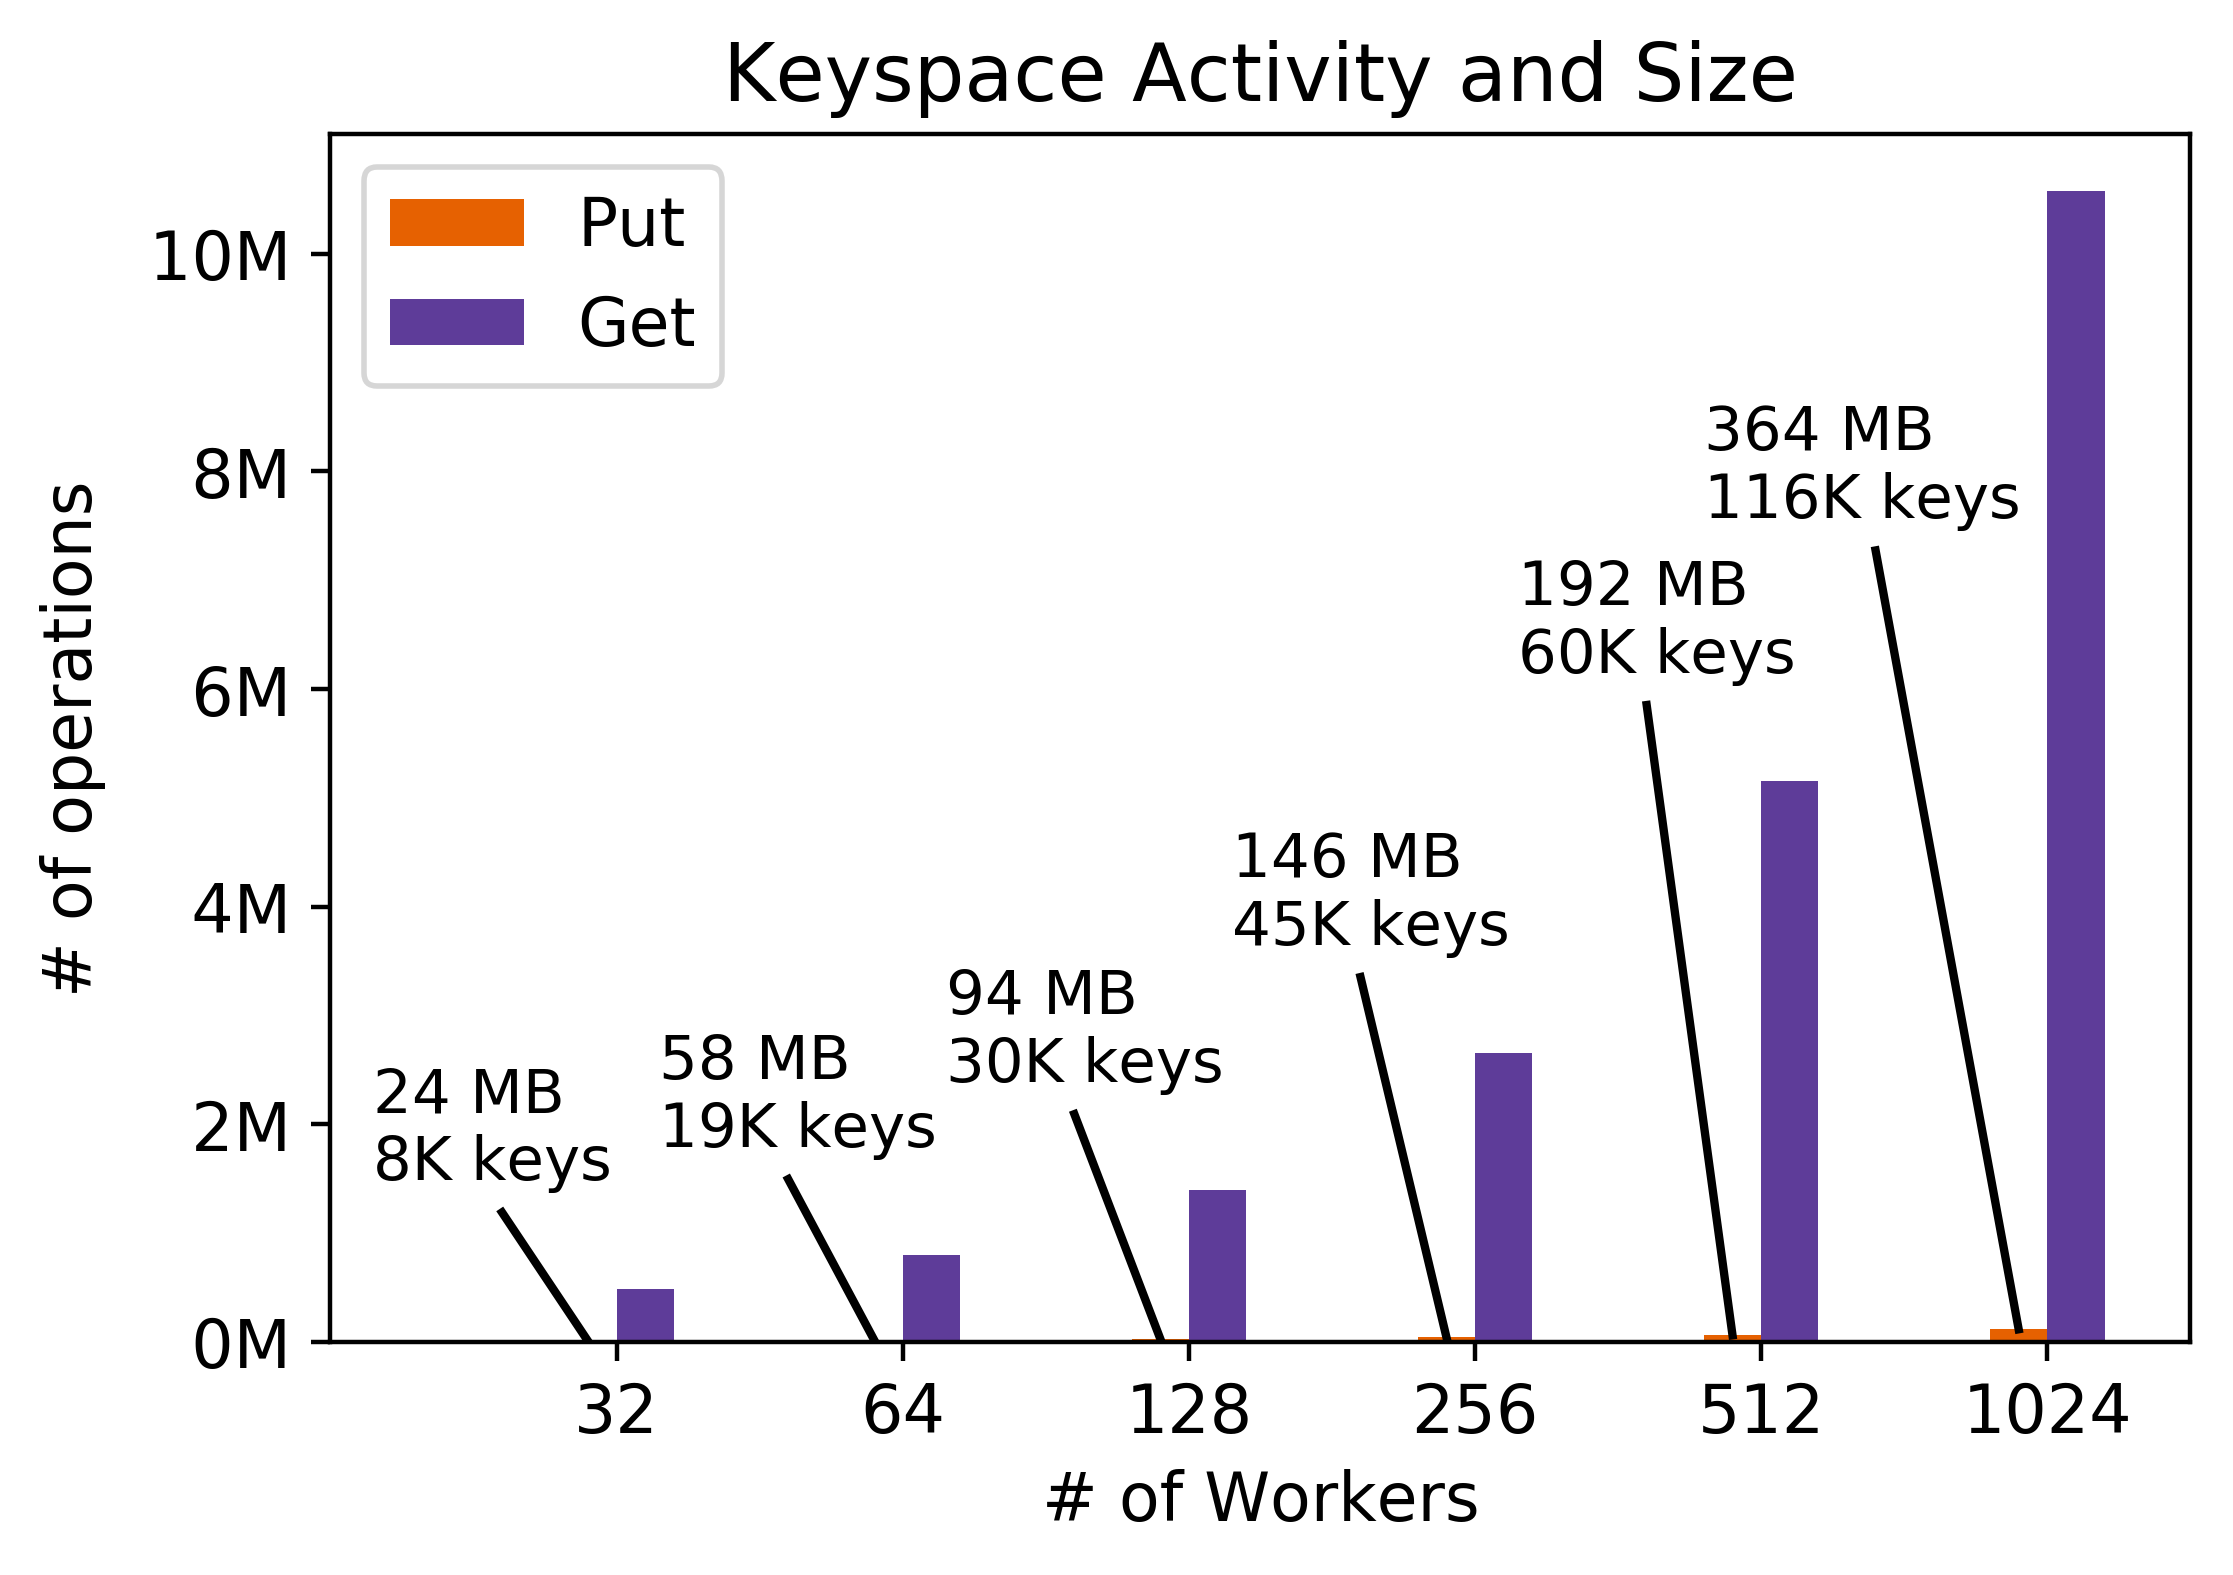
\includegraphics[width=0.45\textwidth]{figures/methodology-keyspace.png}\\
  \caption{The keyspace size is small (numbers above bars) but must
  satisfy many reads as workers calculate new segments. The active keyspace is
  difficult to predict a priori but the optimal load balancing strategy strikes a
  good balance between preformance and utilization. 
  \label{fig:methodology-keyspace}}
\end{figure}

\begin{figure}[tbh]
  \noindent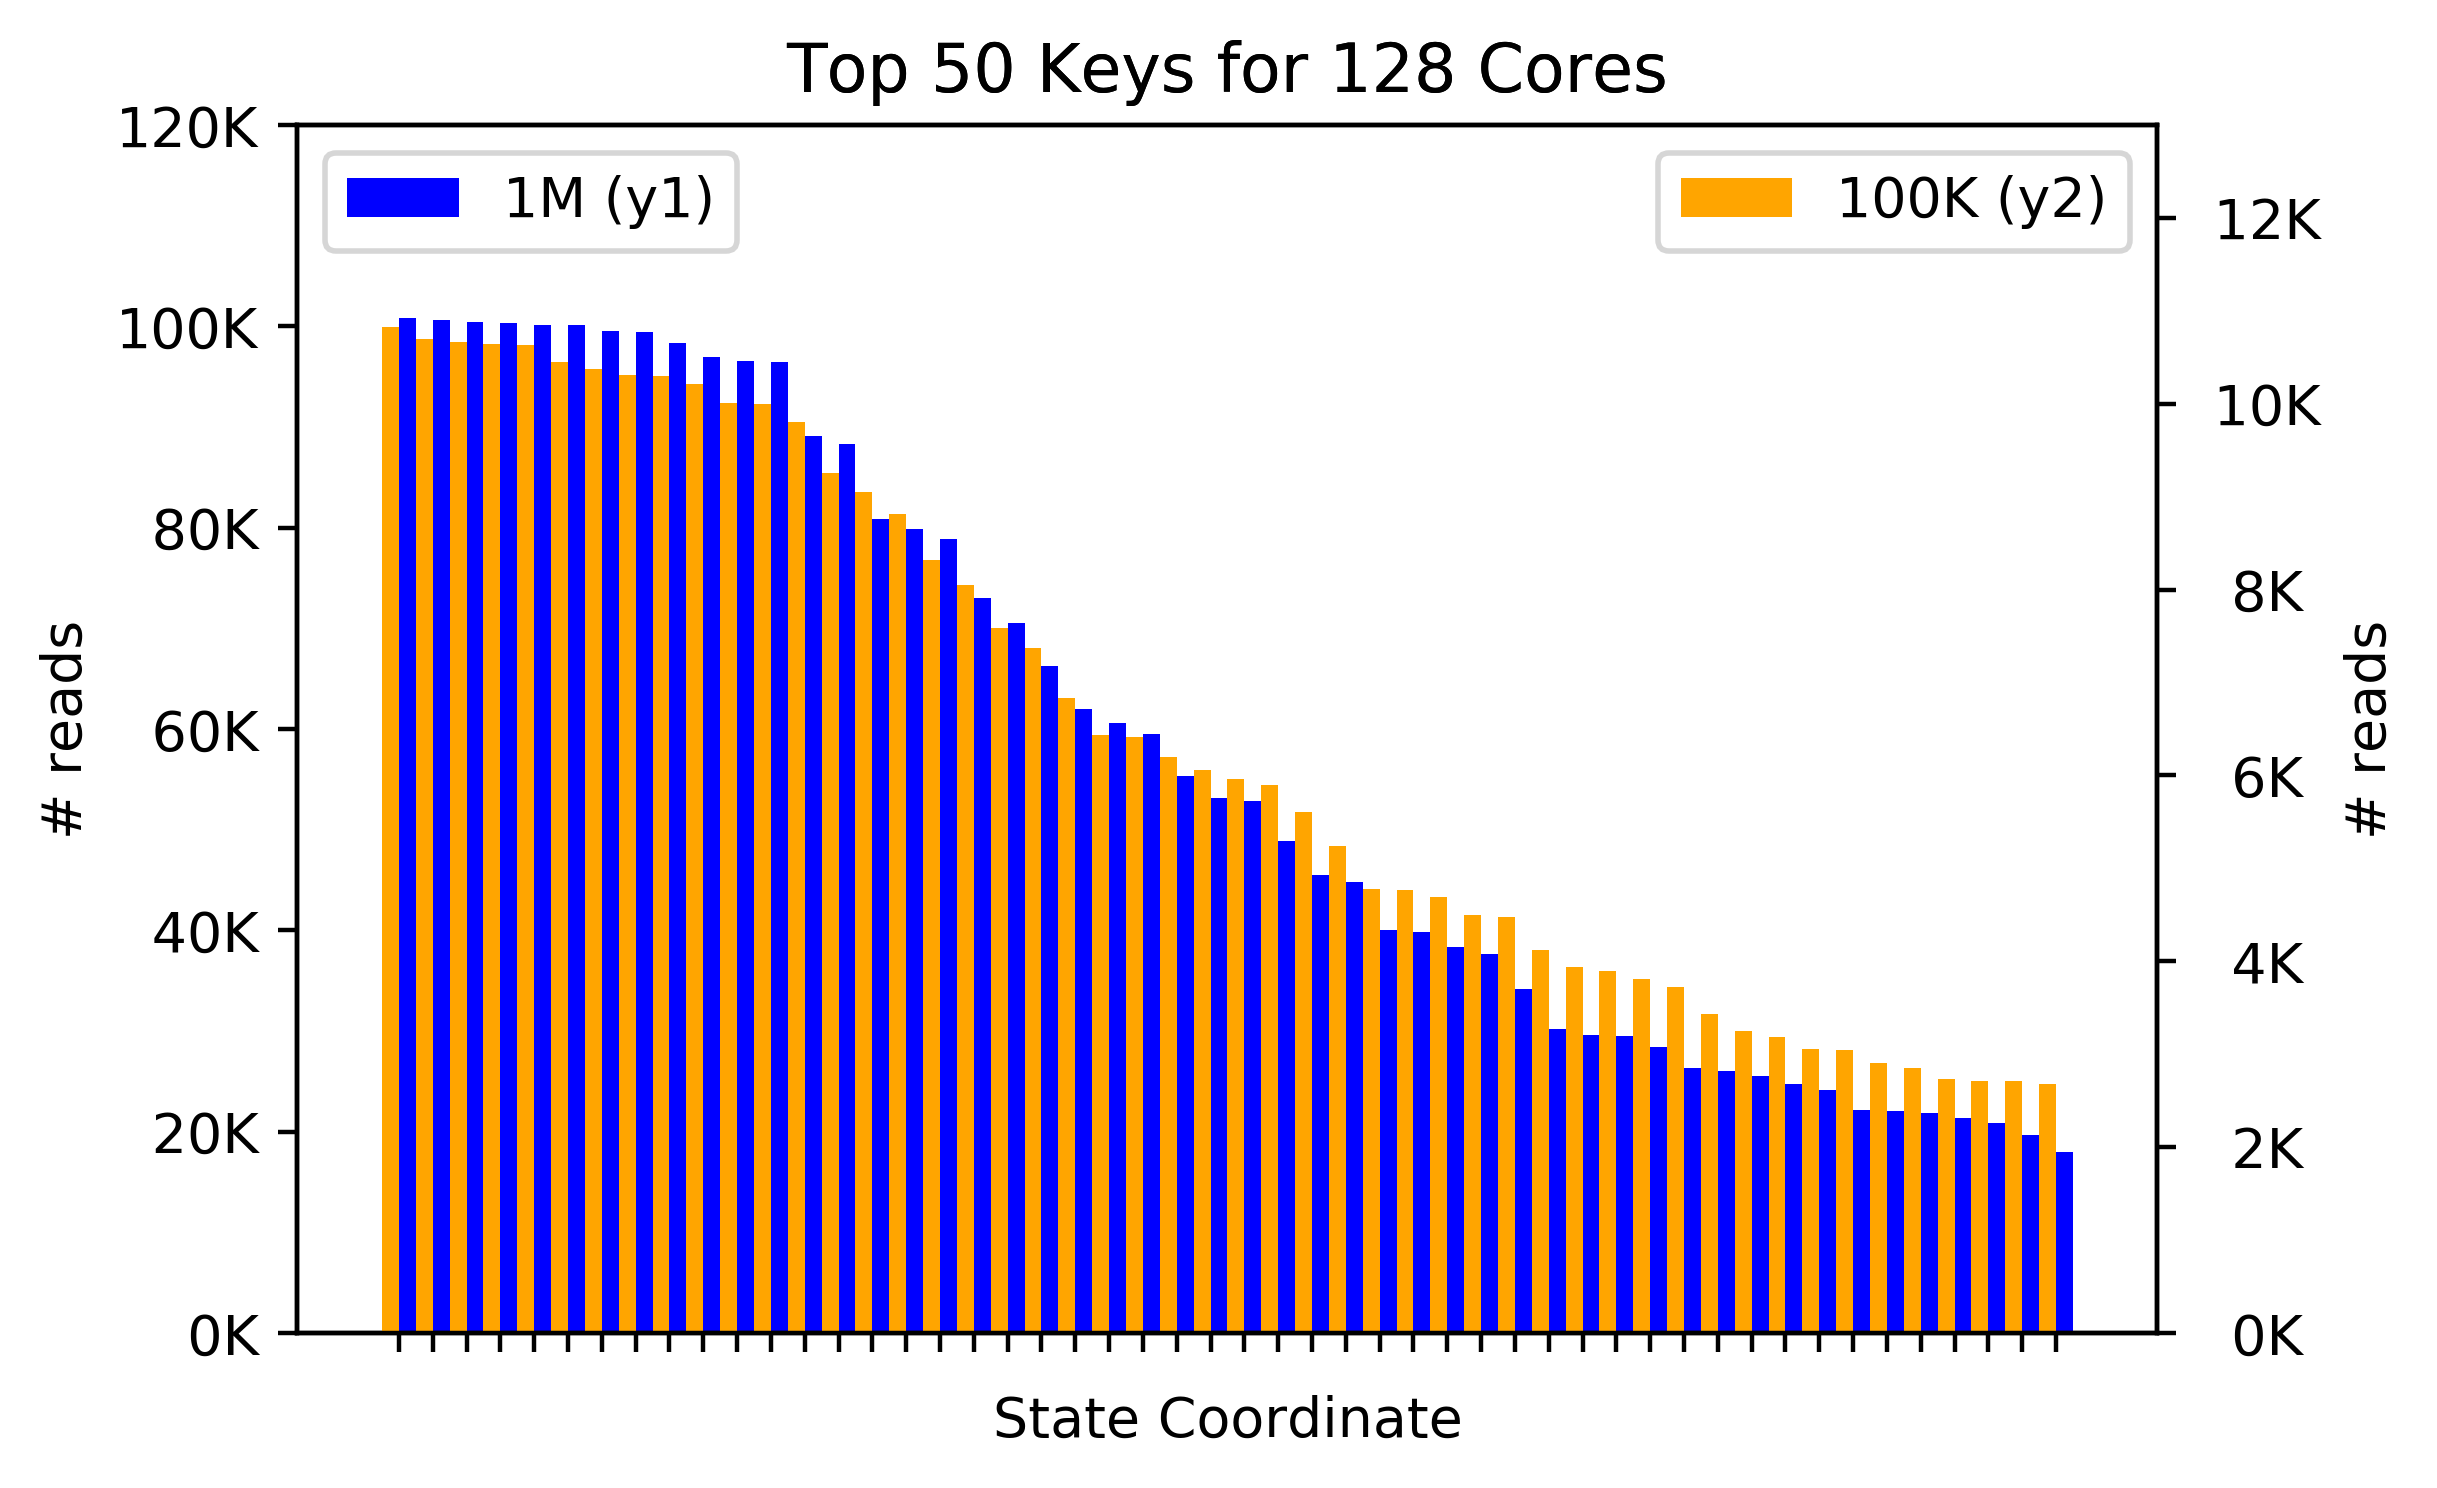
\includegraphics[width=0.45\textwidth]{figures/methodology-keys.png}\\
  \caption{The keyspace imbalance is due to workers generating deep
  trajectories and reading the same coordinates. Over time, the accesses get
  dispersed across different coordinates resulting in some keys being more
  popular than others.\label{fig:methodology-keys}}
\end{figure}

